\documentclass[a4paper,12pt]{report}
\usepackage[utf8]{inputenc}
\usepackage[greek,english]{babel}  % For Greek and English languages
\usepackage{graphicx}              % For including images like logos
\usepackage{tocloft}               % For customizing table of contents

\usepackage[left=2.5cm,right=2cm,top=2cm,bottom=2cm]{geometry}

\usepackage{tabularx} % for adjusting column widths
\usepackage{booktabs} % For better-looking tables
\usepackage[table]{xcolor} % For color in tables
\usepackage{colortbl} % For color in tables
\usepackage{alphabeta}
\usepackage{babelbib}                    
\usepackage{amsmath}
\usepackage{mathrsfs}
\usepackage{rsfso}
\usepackage{xcolor}
\usepackage{csvsimple}
\usepackage{float} % for [H] placement specifier
\usepackage{parskip}
\setlength{\parskip}{\baselineskip}
\setlength{\parindent}{0pt}
\usepackage{circuitikz}
\usepackage{chngcntr}
\usepackage{array} % for custom column widths
\usepackage{enumitem}
\setlist{noitemsep} % Χωρίς επιπλέον κενά μεταξύ των αντικειμένων της λίστας
\usepackage{appendix}
\usepackage{csquotes}
\usepackage{hyperref}
\usepackage{float}

\usepackage[fixlanguage]{babelbib} % Add fixlanguage option here

\newcommand{\gr}{\selectlanguage{greek}}  % Switch to Greek
\newcommand{\en}{\selectlanguage{english}}  % Switch to English


\begin{document}

\gr

% Cover Page
\begin{titlepage}
    \centering
    
    % Add your university/institution logo if needed
    
\includegraphics[width=0.25\textwidth]{figures/emp_logo.png}
    
    \vspace{1cm}
    
    \textbf{\LARGE Εθνικό Μετσόβιο Πολυτεχνείο}

    \vspace{0.05cm}
    
    \textbf{\Large ΔΠΜΣ Παραγωγή και Διαχείριση Ενέργειας}

    \textbf{Σχολή Ηλεκτρολόγων Μηχανικών και Μηχανικών Υπολογιστών}

    \vspace{2cm}

    \textbf{Μεταπτυχιακή Διπλωματική Εργασία}

    \vspace{1cm}

    \textbf{\Large Βελτιστοποίηση λειτουργίας μικροδικτύου με μονάδα
κυψελών καυσίμου υδρογόνου, κατανεμημένες
παραγωγές, αποθήκευση και ευέλικτα φορτία}
    
    \vspace{1cm}
    
    \textbf{\Large Γεωργία Καραταράκη}
    
    \vspace{1.2cm}
    
    \textbf{Επιβλέπων:\\ Ομότιμος Καθηγητής ΕΜΠ \\ Νικόλαος Χατζηαργυρίου}
    
    \vspace{4cm}
    
    \textbf{\large Αθήνα, Οκτώβριος, 2024} % Replace with your graduation month and year
    
    \vfill
           
\end{titlepage}

\newpage  % Create a new page
\thispagestyle{empty}  % Suppress page numbering on this page
\mbox{}  % Insert an empty box to ensure the page exists but is blank

% Start with Roman numbering for the front matter
\pagenumbering{roman}

% Σύνοψη
\chapter*{Σύνοψη}
\addcontentsline{toc}{chapter}{Σύνοψη}  % Add Περίληψη to the table of contents
Στην εργασία αυτή μελετάται μία μεθοδολογία βελτιστοποίησης της λειτουργίας ενός μικροδικτύου. Το μικροδίκτυο αυτό περιλαμβάνει μονάδα κυψελών καυσίμου (υδρογόνου), κατανεμημένες παραγωγές (ανεμογεννήτριες, φωτοβολταϊκά πάνελ), μονάδες αποθήκευσης ηλεκτρισμού και ευέλικτα φορτία. Εξετάζεται η λειτουργία του μικροδικτύου τόσο σε αυτόνομη \en (islanded) \gr όσο και σε διασυνδεδέμενη \en (grid-connected) \gr κατάσταση. Μελετώνται επίσης διάφορα σενάρια για την τιμή πώλησης και αγοράς της ενέργειας καθώς και για τις μεταβολές της ζήτησης. Η βελτιστοποίηση αφορά την ελαχιστοποίηση του συνολικού κόστους λειτουργίας του μικροδικτύου με οικονομικούς όρους. Τέλος, πραγματοποιείται μία εκτίμηση του ποσού εκπομπών αέριων ρύπων στο βέλτιστο σημείο λειτουργίας του μικροδικτύου. Η επίλυση του προβλήματος βελτιστοποίησης γίνεται στην \en python \gr με χρήση του επιλύτη \en gurobi). \gr

\newpage  % Create a new page
\thispagestyle{empty}  % Suppress page numbering on this page
\mbox{}  % Insert an empty box to ensure the page exists but is blank

% Greek abstract (Περίληψη)
\chapter*{Περίληψη}
\addcontentsline{toc}{chapter}{Περίληψη}  % Add Περίληψη to the table of contents
Your Greek abstract text here...

% Greek keywords section (Λέξεις Κλειδιά)
\noindent\textbf{Λέξεις Κλειδιά:} Your Greek keywords here...

\newpage  % Create a new page
\thispagestyle{empty}  % Suppress page numbering on this page
\mbox{}  % Insert an empty box to ensure the page exists but is blank

% Abstract in English
\en
\chapter*{Abstract}
\addcontentsline{toc}{chapter}{Abstract}  % Add Abstract to the table of contents
Your abstract text in English here...

% Keywords section (after the abstract)
\noindent\textbf{Keywords:} Your keywords in English here...

\newpage  % Create a new page
\thispagestyle{empty}  % Suppress page numbering on this page
\mbox{}  % Insert an empty box to ensure the page exists but is blank

% Acknowledgments
\gr
\chapter*{Ευχαριστίες}
\addcontentsline{toc}{chapter}{Ευχαριστίες}  % Add Ευχαριστίες to the table of contents
Your acknowledgments in Greek here...

\newpage  % Create a new page
\thispagestyle{empty}  % Suppress page numbering on this page
\mbox{}  % Insert an empty box to ensure the page exists but is blank

% Table of contents, list of figures, and tables
\addcontentsline{toc}{chapter}{Περιεχόμενα}  % Add Table of Contents to TOC
\tableofcontents

\newpage  % Create a new page
\thispagestyle{empty}  % Suppress page numbering on this page
\mbox{}  % Insert an empty box to ensure the page exists but is blank

\addcontentsline{toc}{chapter}{Κατάλογος Σχημάτων}  % Add List of Figures to TOC
\listoffigures

\newpage  % Create a new page
\thispagestyle{empty}  % Suppress page numbering on this page
\mbox{}  % Insert an empty box to ensure the page exists but is blank

\addcontentsline{toc}{chapter}{Κατάλογος Πινάκων}  % Add List of Tables to TOC
\listoftables

% "Εισαγωγή" as an unnumbered chapter and add to the table of contents
\chapter*{Εισαγωγή}
\addcontentsline{toc}{chapter}{Εισαγωγή}
Όσο περίεργο κι αν μας ακούγεται, η πρόσβαση σε πηγές ηλεκτρικής ενέργειας για κάποιους εκατομμύρια ανθρώπους τη σήμερον ημέρα αποτελεί πολυτέλεια. Συγκεκριμένα, σύμφωνα με πηγές, περισσότερο από ένα δισεκατομμύριο άνθρωποι παγκοσμίως δεν έχουν πρόσβαση σε ηλεκτρική ενέργεια σήμερα. 
Οι λόγοι είναι σίγουρα οικονομικοί, πολιτικοί αλλά και τεχνικοί. Στα πλαίσια αυτού έχουν εμφανιστεί σε πολλές απομακρυσμένες περιοχές τα λεγόμενα μικροδίκτυα. 

% Now switching to Arabic numbering for the main content
\clearpage
\pagenumbering{arabic}

% Main content starts here with Arabic numbering and numbered chapters
\gr
\chapter{Εισαγωγή στα Μικροδίκτυα}
Τα μικροδίκτυα αποτελούν μια καινοτόμο προσέγγιση στη διαχείριση και διανομή ηλεκτρικής ενέργειας, συμβάλλοντας σημαντικά στη μετάβαση σε ένα βιώσιμο και αποδοτικό ενεργειακό σύστημα. Περιλαμβάνουν τη σύνδεση κατανεμημένων ενεργειακών πόρων (\en Distributed Energy Resources - DERs), \gr όπως φωτοβολταϊκά συστήματα, ανεμογεννήτριες, κυψέλες καυσίμου και συστήματα αποθήκευσης ενέργειας, σε ένα ολοκληρωμένο σύστημα. Σε αντίθεση με τα παραδοσιακά δίκτυα, τα μικροδίκτυα διαχειρίζονται την παραγωγή και κατανάλωση ενέργειας σε τοπικό επίπεδο και μπορούν να λειτουργούν είτε συνδεδεμένα με το κεντρικό δίκτυο (\en grid-connected) είτε αυτόνομα (\en islanded). Αυτή η ευελιξία παρέχει πολλαπλά οφέλη, όπως αυξημένη ενεργειακή αποδοτικότητα, βελτιωμένη αξιοπιστία και μείωση των περιβαλλοντικών επιπτώσεων. Είναι ιδανικά για απομακρυσμένες ή απομονωμένες περιοχές, όπου η πρόσβαση στο κεντρικό δίκτυο είναι δύσκολη ή μη βιώσιμη.

\section{Δομή Μικροδικτύων} 
Η δομή ενός μικροδικτύου περιλαμβάνει τρία κύρια συστατικά: \begin{itemize} 
    \item \textbf{Κατανεμημένες Πηγές Ενέργειας (\en DERs)}, όπως ανανεώσιμες πηγές (π.χ. φωτοβολταϊκά, ανεμογεννήτριες) και συστήματα αποθήκευσης (π.χ. μπαταρίες, υδρογόνο). 
    \\
    \item \textbf{Φορτία}, τα οποία μπορεί να είναι σταθερά ή ελεγχόμενα, ανάλογα με τις ανάγκες και την ευελιξία του μικροδικτύου. 
    \\
    \item \textbf{Συστήματα Ελέγχου}, που διαχειρίζονται τη ροή ενέργειας, προσαρμόζουν την παραγωγή στις ανάγκες κατανάλωσης και εξασφαλίζουν την ασφαλή και αποδοτική λειτουργία. 
\end{itemize}

\section{Λειτουργία Μικροδικτύων} 
Τα μικροδίκτυα μπορούν να λειτουργούν είτε σε σύνδεση με το κεντρικό δίκτυο είτε αυτόνομα. Όταν είναι συνδεδεμένα, υποστηρίζουν το κεντρικό δίκτυο προσφέροντας υπηρεσίες όπως εξισορρόπηση φορτίου και υποστήριξη συχνότητας, διασφαλίζοντας τη σταθερότητα του συστήματος. Όταν λειτουργούν αυτόνομα, αποσυνδέονται από το κεντρικό δίκτυο και βασίζονται αποκλειστικά στους τοπικούς ενεργειακούς πόρους για την κάλυψη των αναγκών τους. Αυτή η δυνατότητα τα καθιστά ιδιαίτερα χρήσιμα σε περιπτώσεις διακοπών ρεύματος ή βλαβών, επιτρέποντας την ενεργειακή αυτονομία. Η τοπική διαχείριση των ενεργειακών πόρων συμβάλλει στη βελτιστοποίηση της χρήσης τους, μειώνοντας τις απώλειες μεταφοράς που είναι συχνές στα μεγάλα δίκτυα.

\section{Πλεονεκτήματα Μικροδικτύων} 
Τα μικροδίκτυα προσφέρουν πολλαπλά πλεονεκτήματα:
\begin{itemize}
    \item \textbf{Ενεργειακή αποδοτικότητα:} Η τοπική παραγωγή μειώνει τις απώλειες μεταφοράς, ενώ η ενσωμάτωση ανανεώσιμων πηγών μειώνει την εξάρτηση από συμβατικές μονάδες παραγωγής. 
    \\
    \item \textbf{Περιβαλλοντική βιωσιμότητα}: Η χρήση ανανεώσιμων πηγών και αποθήκευσης ενέργειας μειώνει τις εκπομπές αερίων του θερμοκηπίου, συμβάλλοντας στην προώθηση ενός πιο βιώσιμου ενεργειακού μέλλοντος.
    \\
    \item \textbf{Αξιοπιστία:} Η δυνατότητα αυτόνομης λειτουργίας ενισχύει την ανθεκτικότητα των δικτύων σε διακοπές ή βλάβες, διασφαλίζοντας την ενεργειακή παροχή σε κρίσιμες υποδομές.
    \\
    \item \textbf{Οικονομία:} Η τοπική παραγωγή και κατανάλωση ενέργειας μειώνει την ανάγκη για μεγάλες κεντρικές μονάδες παραγωγής και τις σχετικές δαπάνες μεταφοράς, καθιστώντας τα μικροδίκτυα οικονομικά βιώσιμα, ειδικά για απομακρυσμένες περιοχές.
\end{itemize}

\section{Μικροδίκτυα και Ενεργειακή Μετάβαση} 
Τα μικροδίκτυα θεωρούνται βασικός παράγοντας για την ενεργειακή μετάβαση προς ένα πιο βιώσιμο και αποκεντρωμένο σύστημα. Η ενσωμάτωση ανανεώσιμων πηγών και συστημάτων αποθήκευσης μειώνει την εξάρτηση από τα ορυκτά καύσιμα και ενισχύει την ενεργειακή αυτονομία σε τοπικό επίπεδο. Οι τεχνολογίες έξυπνης διαχείρισης επιτρέπουν τη βελτιστοποίηση της παραγωγής και κατανάλωσης, ενισχύοντας την αποδοτικότητα και μειώνοντας τις απώλειες. Συνολικά, τα μικροδίκτυα προωθούν την ενεργειακή βιωσιμότητα, την οικονομική αποδοτικότητα και τη βελτιωμένη ανθεκτικότητα του ενεργειακού συστήματος. 
\gr
\chapter{Εισαγωγή στη Βελτιστοποίηση}
Η βελτιστοποίηση αποτελεί θεμελιώδες πεδίο των μαθηματικών και της επιστήμης των υπολογιστών, το οποίο ασχολείται με την εύρεση της βέλτιστης λύσης για προβλήματα που σχετίζονται με την αποδοτική διαχείριση πόρων, τη λήψη αποφάσεων και τη βελτίωση της λειτουργίας συστημάτων. Στόχος της βελτιστοποίησης είναι η μεγιστοποίηση ή η ελαχιστοποίηση μιας αντικειμενικής συνάρτησης, συνήθως υπό συγκεκριμένους περιορισμούς που αφορούν τις φυσικές, οικονομικές ή τεχνολογικές παραμέτρους του συστήματος που μελετάται.

\section{Βασικές Αρχές Βελτιστοποίησης}
Στη βελτιστοποίηση, το πρόβλημα διατυπώνεται με μια μαθηματική μοντελοποίηση, η οποία περιλαμβάνει την αντικειμενική συνάρτηση που πρέπει να μεγιστοποιηθεί ή να ελαχιστοποιηθεί και ένα σύνολο περιορισμών που θέτουν τα όρια μέσα στα οποία πρέπει να βρεθεί η λύση. Οι βασικές αρχές της βελτιστοποίησης μπορούν να διακριθούν σε διάφορους τύπους ανάλογα με τη φύση του προβλήματος και τα χαρακτηριστικά των δεδομένων:
\begin{itemize}
    \item \textbf{Γραμμική βελτιστοποίηση:} Στη γραμμική βελτιστοποίηση, η αντικειμενική συνάρτηση και οι περιορισμοί είναι γραμμικές σχέσεις των μεταβλητών. Το πρόβλημα μπορεί να επιλυθεί με μεθόδους όπως ο απλός αλγόριθμος (Simplex) ή οι αλγόριθμοι εσωτερικού σημείου. Αυτή η κατηγορία είναι ιδιαίτερα χρήσιμη σε προβλήματα όπου οι σχέσεις ανάμεσα στις μεταβλητές είναι γραμμικές και το ζητούμενο είναι η μεγιστοποίηση ή ελαχιστοποίηση μιας απλής συνάρτησης κόστους ή κέρδους.
    \\
    \item \textbf{Μη γραμμική βελτιστοποίηση:} Σε αυτή την κατηγορία, είτε η αντικειμενική συνάρτηση είτε οι περιορισμοί είναι μη γραμμικοί. Η επίλυση τέτοιων προβλημάτων είναι συνήθως πιο σύνθετη από τα γραμμικά προβλήματα, καθώς απαιτούνται ειδικές τεχνικές για την αντιμετώπιση της πολυπλοκότητας που δημιουργούν οι μη γραμμικές σχέσεις.
    \\
    \item \textbf{Ακέραια βελτιστοποίηση:} Η ακέραια βελτιστοποίηση αναφέρεται σε προβλήματα όπου οι μεταβλητές απόφασης μπορούν να λάβουν μόνο ακέραιες τιμές. Τέτοια προβλήματα εμφανίζονται συχνά σε περιπτώσεις όπου οι αποφάσεις είναι δυαδικές ή διακριτές (π.χ., να επιλέξεις ή να απορρίψεις μια επιλογή).
    \\
    \item \textbf{Στοχαστική βελτιστοποίηση:} Σε αυτόν τον τύπο βελτιστοποίησης, ορισμένες παράμετροι του προβλήματος εμπεριέχουν αβεβαιότητα και διατυπώνονται ως τυχαίες μεταβλητές με πιθανότητες. Η στοχαστική βελτιστοποίηση χρησιμοποιείται για την αντιμετώπιση προβλημάτων όπου υπάρχει αβεβαιότητα στις τιμές των παραμέτρων, όπως για παράδειγμα σε προβλέψεις ζήτησης ή παραγωγής ενέργειας.
    \\
    \textbf{Ντετερμινιστική βελτιστοποίηση:} Η ντετερμινιστική βελτιστοποίηση αναφέρεται σε προβλήματα όπου όλες οι παράμετροι του συστήματος είναι γνωστές και σταθερές, χωρίς αβεβαιότητα. Στα ντετερμινιστικά προβλήματα, τα δεδομένα του συστήματος είναι σαφή και η λύση εξαρτάται αποκλειστικά από αυτές τις γνωστές παραμέτρους. Τα γραμμικά και μη γραμμικά προβλήματα συχνά ανήκουν σε αυτή την κατηγορία όταν δεν εμπεριέχουν αβεβαιότητα.
    \\
    \item \textbf{Δυναμική βελτιστοποίηση:} Η δυναμική βελτιστοποίηση ασχολείται με προβλήματα όπου οι παράμετροι ή οι περιορισμοί αλλάζουν με τον χρόνο. Σε αυτά τα προβλήματα, η λύση πρέπει να λαμβάνει υπόψη τη χρονική εξέλιξη του συστήματος και να προσαρμόζεται ανάλογα.
\end{itemize}

\section{Αλγόριθμοι Βελτιστοποίησης}
Η βελτιστοποίηση αποτελεί κρίσιμη διαδικασία σε ένα ευρύ φάσμα βιομηχανικών και ερευνητικών εφαρμογών. Η αποτελεσματική επίλυση προβλημάτων βελτιστοποίησης συχνά βασίζεται σε λογισμικά εργαλεία που εφαρμόζουν προηγμένους αλγόριθμους, προκειμένου να επιτευχθούν τα επιθυμητά αποτελέσματα με αποδοτικότητα και ακρίβεια.

Ένα από τα πιο δημοφιλή και ευρέως χρησιμοποιούμενα εμπορικά εργαλεία βελτιστοποίησης είναι το \en Gurobi, \gr το οποίο προσφέρει ισχυρούς αλγορίθμους για την επίλυση γραμμικών, μη γραμμικών και ακέραιων προβλημάτων. Το \en Gurobi \gr είναι γνωστό για την ταχύτητα και την αξιοπιστία του, και χρησιμοποιείται ευρέως τόσο στην ακαδημαϊκή έρευνα όσο και σε βιομηχανικές εφαρμογές, όπως η διαχείριση πόρων και η βελτιστοποίηση εφοδιαστικής αλυσίδας.

Άλλοι γνωστοί επιλύτες, όπως το \en CPLEX \gr και το \en FICO Xpress, \gr προσφέρουν παρόμοιες δυνατότητες και χρησιμοποιούνται για τη λύση σύνθετων προβλημάτων βελτιστοποίησης σε διάφορους τομείς, συμπεριλαμβανομένων των χρηματοοικονομικών, της ενέργειας και των μεταφορών. Τα εργαλεία αυτά ενσωματώνουν αλγόριθμους όπως ο \en Simplex \gr για γραμμικά προβλήματα και οι αλγόριθμοι εσωτερικού σημείου για πιο πολύπλοκα μη γραμμικά συστήματα.

Η χρήση εμπορικών λογισμικών για τη βελτιστοποίηση επιτρέπει την επίλυση προβλημάτων μεγάλης κλίμακας, εξασφαλίζοντας ταχύτητα και ακρίβεια στα αποτελέσματα, γεγονός που τα καθιστά απαραίτητα εργαλεία για βιομηχανίες που απαιτούν βέλτιστη διαχείριση πόρων και κόστος λειτουργίας.

\section{Εφαρμογές Βελτιστοποίησης}
Η βελτιστοποίηση βρίσκει εφαρμογή σε ένα ευρύ φάσμα τομέων:
\begin{itemize}
    \item \textbf{Βιομηχανία:} Βελτιστοποίηση της παραγωγής, της διαχείρισης πόρων και της εφοδιαστικής αλυσίδας για τη μείωση του κόστους και την αύξηση της αποδοτικότητας.
    \\
    \item \textbf{Ενέργεια:} Βελτιστοποίηση των ενεργειακών συστημάτων, όπως η διαχείριση ανανεώσιμων πηγών ενέργειας και η αποθήκευση ενέργειας, για την ελαχιστοποίηση του κόστους και την αποδοτική χρήση των πόρων.
    \\
    \item \textbf{Οικονομικά:} Βελτιστοποίηση των επενδυτικών στρατηγικών και της διαχείρισης κινδύνου, λαμβάνοντας υπόψη τους περιορισμούς κεφαλαίου και την αβεβαιότητα των αγορών.
    \\
    \item \textbf{Μεταφορές:} Βελτιστοποίηση δρομολογίων και διαχείρισης αποθεμάτων για την ελαχιστοποίηση του κόστους μεταφοράς και την καλύτερη εξυπηρέτηση των πελατών.
\end{itemize}





  
\gr
\chapter{Το Υδρογόνο ως Ενεργειακός Πόρος}

\section{Εισαγωγή}
Το υδρογόνο αναδεικνύεται ως ένας από τους πιο σημαντικούς ενεργειακούς φορείς για την ενεργειακή μετάβαση προς ένα βιώσιμο μέλλον. Η δυνατότητα του υδρογόνου να λειτουργεί ως φορέας καθαρής ενέργειας το καθιστά ιδανικό για την επίτευξη των παγκόσμιων στόχων για τη μείωση των εκπομπών διοξειδίου του άνθρακα ($CO_2$). Σε αντίθεση με τα ορυκτά καύσιμα, η κατανάλωση υδρογόνου δεν παράγει επιβλαβείς εκπομπές $CO_2$, καθώς το παραγόμενο υποπροϊόν είναι το καθαρό νερό ($H_2O$). Λόγω αυτών των πλεονεκτημάτων, το υδρογόνο θεωρείται ο βασικός ενεργειακός φορέας σε διάφορους τομείς, όπως η βιομηχανία, οι μεταφορές και η παραγωγή ηλεκτρικής ενέργειας.

\section{Παραγωγή Υδρογόνου}
Το υδρογόνο δεν είναι άμεσα διαθέσιμο στη φύση, αλλά πρέπει να παραχθεί μέσω διαδικασιών όπως η ηλεκτρόλυση του νερού ή η αναμόρφωση φυσικού αερίου. Η ηλεκτρόλυση θεωρείται η πιο βιώσιμη μέθοδος παραγωγής πράσινου υδρογόνου, καθώς βασίζεται στη χρήση ανανεώσιμης ηλεκτρικής ενέργειας για τη διάσπαση του νερού ($H_2O$) σε υδρογόνο ($H_2$) και οξυγόνο ($O_2$). Κατά τη διαδικασία αυτή, οι ενεργειακές πηγές, όπως τα φωτοβολταϊκά και οι ανεμογεννήτριες, παρέχουν την απαιτούμενη ηλεκτρική ενέργεια, καθιστώντας το τελικό προϊόν απολύτως καθαρό και φιλικό προς το περιβάλλον.

Εκτός από την ηλεκτρόλυση, το υδρογόνο μπορεί να παραχθεί και μέσω άλλων διαδικασιών, όπως η αναμόρφωση μεθανίου (\en Steam Methane Reforming - SMR), \gr η οποία ωστόσο οδηγεί σε εκπομπές ($CO_2$) και δεν θεωρείται πράσινη μέθοδος. Για την παραγωγή πράσινου υδρογόνου, είναι κρίσιμη η χρήση ανανεώσιμων πηγών ενέργειας, ώστε η όλη διαδικασία να είναι βιώσιμη και φιλική προς το περιβάλλον.

\section{Χρήση Υδρογόνου σε Κυψέλες Καυσίμου}
Οι κυψέλες καυσίμου υδρογόνου αποτελούν την πιο διαδεδομένη τεχνολογία για την αξιοποίηση του υδρογόνου. Στις κυψέλες καυσίμου, το υδρογόνο αντιδρά με το οξυγόνο (συνήθως από τον αέρα) για την παραγωγή ηλεκτρικής ενέργειας, θερμότητας και νερού, χωρίς την εκπομπή ρυπογόνων αερίων. Η αντίδραση αυτή είναι ηλεκτροχημική και δεν εμπλέκει καύση, γεγονός που την καθιστά εξαιρετικά αποδοτική και φιλική προς το περιβάλλον. Η βασική λειτουργία μιας κυψέλης καυσίμου βασίζεται στην αρχή του ηλεκτροχημικού στοιχείου, όπου η χημική ενέργεια του υδρογόνου μετατρέπεται απευθείας σε ηλεκτρική ενέργεια.

Οι κυψέλες καυσίμου παρουσιάζουν διάφορους τύπους, ανάλογα με τη θερμοκρασία λειτουργίας και τα υλικά που χρησιμοποιούνται. Οι πιο κοινές κυψέλες είναι οι Πολυμερικές Κυψέλες Καυσίμου (\en PEMFCs), \gr οι οποίες λειτουργούν σε χαμηλές θερμοκρασίες και χρησιμοποιούνται σε πολλές εφαρμογές, συμπεριλαμβανομένων των μεταφορών και των μικροδικτύων. Επίσης, υπάρχουν οι Κυψέλες Καυσίμου Υψηλής Θερμοκρασίας, όπως οι Κυψέλες Οξειδίων Στερεάς Κατάστασης (\en SOFCs), \gr οι οποίες είναι κατάλληλες για βιομηχανικές εφαρμογές λόγω της υψηλής απόδοσης και θερμοκρασίας λειτουργίας τους.

\section{Ο Ρόλος των Κυψέλων Καυσίμου στα Μικροδίκτυα}
Στα μικροδίκτυα, οι κυψέλες καυσίμου υδρογόνου διαδραματίζουν καθοριστικό ρόλο στην παροχή καθαρής ενέργειας, ιδιαίτερα όταν οι ανανεώσιμες πηγές, όπως τα φωτοβολταϊκά ή οι ανεμογεννήτριες, δεν παράγουν επαρκή ηλεκτρική ενέργεια λόγω καιρικών συνθηκών ή μειωμένης ζήτησης. Οι κυψέλες καυσίμου παρέχουν ενέργεια κατόπιν ζήτησης, λειτουργώντας συμπληρωματικά με άλλες μονάδες παραγωγής ενέργειας.

Ένα βασικό πλεονέκτημα των κυψέλων καυσίμου είναι η ελαστικότητα στην απόκριση στη ζήτηση. Οι κυψέλες καυσίμου μπορούν να ενεργοποιούνται γρήγορα και να λειτουργούν αποτελεσματικά σε ένα ευρύ φάσμα ισχύος, εξασφαλίζοντας τη συνεχή λειτουργία του μικροδικτύου. Η ενσωμάτωση συστημάτων κυψελών καυσίμου σε ένα μικροδίκτυο προσφέρει επίσης αυξημένη ανθεκτικότητα του δικτύου (\en resilience), \gr καθώς μπορούν να καλύψουν ενεργειακά κενά που προκύπτουν λόγω της διακοπής παροχής από ανανεώσιμες πηγές.

\section{Αποθήκευση και Μεταφορά Υδρογόνου}
Η αποθήκευση του υδρογόνου αποτελεί μια κρίσιμη πρόκληση για τη βέλτιστη αξιοποίησή του ως ενεργειακός φορέας. Το υδρογόνο μπορεί να αποθηκευτεί σε συμπιεσμένη μορφή, υγροποιημένη μορφή ή σε χημικές ενώσεις, όπως τα μεταλλικά υδρίδια. Η συμπιεσμένη αποθήκευση υδρογόνου σε υψηλές πιέσεις (π.χ. \en 350 ή 700 bar) \gr είναι μια κοινή πρακτική, ιδιαίτερα για μικροδίκτυα και μεταφορές, λόγω της σχετικά απλής τεχνολογίας. Από την άλλη, η υγροποίηση υδρογόνου απαιτεί χαμηλές θερμοκρασίες, γεγονός που καθιστά τη διαδικασία ενεργοβόρα, αλλά κατάλληλη για μεγάλες ποσότητες.

Η αποδοτική αποθήκευση του υδρογόνου επιτρέπει στα μικροδίκτυα να αποθηκεύουν την ενέργεια που παράγεται από ανανεώσιμες πηγές κατά τη διάρκεια της ημέρας ή όταν υπάρχει υπερπαραγωγή, για να την χρησιμοποιήσουν αργότερα όταν υπάρχει αυξημένη ζήτηση ή μειωμένη παραγωγή. Έτσι, το υδρογόνο λειτουργεί ως ένας ενεργειακός μεσάζων που επιτρέπει την εξομάλυνση των διακυμάνσεων στην παραγωγή και κατανάλωση ενέργειας, εξασφαλίζοντας τη σταθερότητα του μικροδικτύου.

\gr
\chapter{Υπό Μελέτη Μικροδίκτυο}
Το μικροδίκτυο που εξετάζεται στην παρούσα μελέτη αποτελείται από ανανεώσιμες πηγές ενέργειας και τεχνολογίες αποθήκευσης. Συγκεκριμένα, η παραγωγή ενέργειας προέρχεται από μία συστοιχία φωτοβολταϊκών πάνελ, μία ανεμογεννήτρια, ενώ η αποθήκευση ενέργειας υλοποιείται μέσω συστοιχιών μπαταριών και ενός συστήματος υδρογόνου. Το σύστημα υδρογόνου περιλαμβάνει τρεις κύριες μονάδες: τη μονάδα ηλεκτρόλυσης για την παραγωγή υδρογόνου, τη μονάδα αποθήκευσης και τη μονάδα κυψελών καυσίμου για την παραγωγή ηλεκτρικής ενέργειας. Αυτή η δομή επιτρέπει την ολοκληρωμένη διαχείριση των ανανεώσιμων πηγών, συμβάλλοντας στην ενεργειακή αυτονομία του μικροδικτύου.

Στο πλαίσιο της παρούσας διπλωματικής εργασίας, η λειτουργία του μικροδικτύου προκύπτει από την επίλυση ενός γραμμικού προβλήματος βελτιστοποίησης, όπου λαμβάνονται υπόψη οι περιορισμοί που σχετίζονται με τα χαρακτηριστικά των μονάδων αποθήκευσης και τις απαιτήσεις του συστήματος. Η βελτιστοποίηση επικεντρώνεται στα κόστη λειτουργίας των μονάδων αποθήκευσης, ενώ η παραγωγή ενέργειας από τις ανανεώσιμες πηγές θεωρείται δεδομένη, καθώς οι μονάδες παραγωγής λειτουργούν πάντοτε στο μέγιστο επίπεδο τους, ανάλογα με τις καιρικές συνθήκες. Ο βασικός στόχος είναι να καθοριστεί ποιες μονάδες αποθήκευσης είναι οικονομικά αποδοτικό να ενεργοποιηθούν, ώστε να επιτευχθεί η ελαχιστοποίηση του συνολικού κόστους λειτουργίας του μικροδικτύου.

% Ένα χαρακτηριστικό παράδειγμα λειτουργίας ενός τέτοιου μικροδικτύου είναι το μικροδίκτυο της Ξάνθης, που αναπτύχθηκε στο πλαίσιο του έργου \en X-FLEX \cite{10137658}. \gr Η πλεονάζουσα ενέργεια που παράγεται από τα φωτοβολταϊκά και τις ανεμογεννήτριες χρησιμοποιείται για τη φόρτιση των μπαταριών του συστήματος. Εφόσον οι μπαταρίες είναι πλήρως φορτισμένες, η επιπλέον ενέργεια τροφοδοτεί τη μονάδα ηλεκτρόλυσης για την παραγωγή υδρογόνου, το οποίο αποθηκεύεται σε συμπιεσμένη μορφή σε ειδικές δεξαμενές για μελλοντική χρήση. Σε περίπτωση που και οι μπαταρίες και οι δεξαμενές υδρογόνου είναι πλήρεις, η πλεονάζουσα ενέργεια πωλείται στο δίκτυο.

% Όταν η ζήτηση ενέργειας του μικροδικτύου δεν μπορεί να καλυφθεί από τις ανανεώσιμες πηγές, ενεργοποιείται η αποθηκευμένη ενέργεια. Αρχικά χρησιμοποιούνται οι μπαταρίες, ενώ εάν αυτές εξαντληθούν, το υδρογόνο από τις δεξαμενές μετατρέπεται σε ηλεκτρική ενέργεια μέσω της μονάδας κυψελών καυσίμου. Εάν η αποθηκευμένη ενέργεια δεν επαρκεί για την κάλυψη της ζήτησης, το μικροδίκτυο λαμβάνει ενέργεια από το κεντρικό δίκτυο. Αυτή η διαδικασία δημιουργεί νέες προοπτικές στην αγορά ενέργειας, συμβάλλοντας παράλληλα στη μείωση των εκπομπών αερίων του θερμοκηπίου και στην καταπολέμηση της κλιματικής αλλαγής.

\section{Φωτοβολταϊκό σύστημα}
Η ισχύς εξόδου ενός φωτοβολταϊκού συστήματος υπολογίζεται βάσει της σχέσης \cite{CAU2014820}:
\begin{equation}
    P_{PV}=G\cdot A_{PV} \cdot N_{PV} \cdot η_{PV} \label{P_PV}
\end{equation}
όπου:
\begin{itemize}
  \item[] $P_{PV}$, η ισχύς εξόδου ενός φωτοβολταϊκού συστήματος σε $kW$ 
  \\
  \item[] $G$, η προσπίπτουσα ηλιακή ακτινοβολία σε $W/m^2$ 
  \\
  \item[] $A_{PV}$, η επιφάνεια ενός φωτοβολταϊκού πάνελ σε $m^2$
  \\
  \item[] $N_{PV}$, ο συνολικός αριθμός των πάνελ του φωτοβολταϊκού συστήματος 
  \\
  \item[] $η_{PV}$, η απόδοση ενός ηλιακού πάνελ 
\end{itemize}

Η απόδοση κάθε ηλιακού πάνελ υπολογίζεται ως εξής \cite{CAU2014820}:
\begin{equation}
    \eta_{PV} = \eta_{PV,REF} \cdot \left[ 1 - \alpha \cdot \left( T_{AMB} + G \cdot \frac{NOCT - 20}{800} - T_{REF} \right) \right] \label{\eta_PV}
\end{equation}
όπου:
\begin{itemize}
  \item[] $\eta_{PV}$, η απόδοση ενός ηλιακού πάνελ σε συγκεκριμένες συνθήκες
  \\
  \item[] $\eta_{PV,REF}$, η απόδοση ενός ηλιακού πάνελ όταν $G = 1000 W/m^2$ και $T_{REF}=25^oC$)
  \\
  \item[] $T_{AMB}$, η θερμοκρασία περιβάλλοντος σε $^oC$
  \\
  \item[] α, ο συντελεστής θερμοκρασίας σε $1/K$ 
  \\
  \item[] $NOCT$, η ονομαστική θερμοκρασία λειτουργίας της μονάδας σε $^oC$ 
  \\
  \item[] $T_{REF}$, η θερμοκρασία αναφοράς της μονάδας, $Τ_{REF}=25^oC$ 
\end{itemize}
Τα παραπάνω στοιχεία δίνονται από τον κατασκευαστή της φωτοβολταϊκής μονάδας \cite{sunpower} και καταγράφονται στον Πίνακα \ref{tab:pv_data} \cite{CAU2014820}. 

Για την επίλυση του προβλήματος βελτιστοποίησης θεωρούμε ότι το φωτοβολταϊκό σύστημα λειτουργεί διαρκώς στο \en MPP (Maximum Power Point). \gr Οι παράμετροι που καθορίζουν την απόδοση του φωτοβολταϊκού συστήματος, $η_{PV}$, είναι η ηλιακή ακτινοβολία και η θερμοκρασία περιβάλλοντος. Τα μετεωρολογικά αυτά δεδομένα εξήχθησαν για την περιοχή της νότιας Κρήτης, την ημέρα 23/07/2023 \cite{solcasttoolkit}. 

\section{Ανεμογεννήτρια}
Η ισχύς εξόδου μίας ανεμογεννήτριας υπολογίζεται βάσει της εξίσωσης \cite{mathematical}:
\begin{equation}
    P_{WT} = 
        \begin{cases} 
        0 & 
        \text{αν } v(t) < v_{cut-in} \text{ ή } v(t) \geq v_{\text{\en cut-out}} \\

        \frac{{(v(t) - v_{\text{\en cut-in}})}}{{(v_{\text{\en rated}} - v_{\text{\en cut-in}})}} \cdot P_{rated} & 
        \text{αν } v_{cut-in} \leq v(t) < v_{rated} \\

        P_{rated} & 
        \text{αν } \en v_{rated} \leq v(t) \leq v_{cut-out} \\

        0 & 
        \text{σε κάθε άλλη περίπτωση} 
        \end{cases} 
        \label{P_WT}
\end{equation}

όπου:
\begin{itemize}
    \item[] $P_{WT}$, η ισχύς της ανεμογεννήτριας σε $kW$
    \\
    \item[] $v$, η ταχύτητα του ανέμου σε $m/s$
    \\
    \item[] $v_{cut-in}$, η ταχύτητα εισόδου σε $m/s$
    \\
    \item[] $v_{rated}$, η ονομαστική ταχύτητα σε $m/s$
    \\
    \item[] $v_{cut-out}$, η ταχύτητα εξόδου σε $m/s$
    \\
    \item[] $P_{rated}$, η ονομαστική ισχύς σε $kW$
\end{itemize}

Η ταχύτητα εισόδου, η ταχύτητα εξόδου καθώς και η ονομαστική ισχύς της ανεμογεννήτριας δίνονται από τον κατασκευαστή της ανεμογεννήτριας \cite{CAU2014820}. Η ταχύτητα ανέμου δίνεται από τα μετεωρολογικά που εξήχθησαν για την περιοχή της νότιας Κρήτης, την ημέρα 23/07/2023 \cite{solcasttoolkit}. Συγκεκριμένα ανά ώρα έχουμε μεταβολή στην τιμή της ταχύτητας του ανέμου. Τα δεδομένα αυτά παρουσιάζονται παρακάτω στον Πίνακα \ref{tab:data}.

Λαμβάνοντας λοιπόν τα δεδομένα της ταχύτητας του ανέμου, μπορούμε να κατασκευάσουμε την καμπύλη ισχύος της ανεμογεννήτριας και να λάβουμε την ισχύ εξόδου της μονάδας σε κάθε χρονική στιγμή. Η ανεμογεννήτρια του μικροδικτύου αποτελείται από τρία πτερύγια, είναι κάθετου άξονα και τα χαρακτηριστικά της δίνονται στον Πίνακα \ref{tab:wt_data} \cite{CAU2014820}.

\section{Μπαταρίες}
Η χρήση μπαταριών για την κάλυψη της ζήτησης όταν δεν υπάρχει παραγωγή είναι μία από τις πιο συνηθισμένες λύσεις σε μικροδίκτυα με ανανεώσιμους διεσπαρμένους πόρους. Ο συνδυασμός τους με την αποθήκευση υδρογόνου αποτελεί έναν διαφορετικό τρόπο λειτουργίας που συμβάλλει στην μεγιστοποίηση του χρόνου ζωής των μπαταριών, αλλά και την αποδοτικότητά τους. 

Η ενέργεια που μπορεί να προσφέρει μία μπαταρία εξαρτάται από την κατάσταση φόρτισής της, το λεγόμενο \en "state of charge" (SOC). \gr Αυτό ισούται με τον λόγο της αποθηκευμένης ενέργειας συναρτήσει της ονομαστικής χωρητικότητας της μπαταρίας και υπολογίζεται παρακολουθώντας την ισχύ φόρτισης και εκφόρτισης της μπαταρίας μέσα στον χρόνο \cite{CAU2014820}:

\begin{equation}
    SOC(t)=SOC(t-1)+\frac{(P_{B,CH}(t) \cdot η_{B,CH}-P_{B,DIS}(t) \cdot η_{B,DIS}) \cdot Δt}{Ν_{Β}U_{Β}Q_{Β}} \label{SOC}
\end{equation}
όπου:
\begin{itemize}
  \item[] $P_{B,CH}(t)$, η ισχύς φόρτισης την ώρα t σε $W$
  \\
  \item[] $P_{B,DIS}(t)$, η ισχύς εκφόρτισης την ώρα t σε $W$
  \\
  \item[] $η_{B,CH}$, η απόδοση της μπαταρίας κατά την φόρτιση 
  \\
  \item[] $η_{B,DIS}$, η απόδοση της μπαταρίας κατά την εκφόρτιση 
  \\
  \item[] $Δt$, το χρονικό βήμα μελέτης στάθμης φόρτισης, το οποίο ισούται με 1 $h$
  \\
  \item[] $N_B$, ο αριθμός των μπαταριών 
  \\
  \item[] $Q_B$, η ονομαστική χωρητικότητα της μπαταρίας σε $Ah$ 
  \\
  \item[] $U_B$, η ονομαστική τάση της μπαταρίας σε $V$ 
  \\
\end{itemize}

Το σύστημα μπαταριών αποτελείται από συστοιχίες μπαταριών μολύβδου οξέος και τα χαρακτηριστικά του καταγράφονται στον Πίνακα \ref{tab:bat_data} \cite{CAU2014820}.

Το κόστος λειτουργίας και συντήρησης της συστοιχίας μπαταριών δεν υπολογίζεται στην παρούσα διπλωματική εργασία. Θεωρείται ότι μεγαλύτερη βαρύτητα έχει ο εκτιμώμενος χρόνος ζωής του συστήματος, ο οποίος υπολογίζεται τόσο για την φόρτιση όσο και για την εκφόρτιση σύμφωνα με τις παρακάτω εξισώσεις αντίστοιχα:  
    \begin{equation}
        L_{B,CH} = \frac{N_B U_B Q_B}{P_{B,CH}(t)}N_{CYCLES} \label{L_B_CH}
    \end{equation}
    \begin{equation}
        L_{B,DIS} = \frac{N_B U_B Q_B}{P_{B,DIS}(t)/η_{B,DIS}}N_{CYCLES} \label{L_B_DIS}
    \end{equation}
όπου:
\begin{itemize}
    \item[] $L_{B,CH}$, ο χρόνος ζωής της μπαταρίας κατά την φόρτιση σε $h$
    \\
    \item[] $L_{B,DIS}$, ο χρόνος ζωής της μπαταρίας κατά την εκφόρτιση σε $h$
    \\
    \item[] $N_{CYCLES}$, ισοδύναμοι κύκλοι φόρτισης και εκφόρτισης της μπαταρίας 
\end{itemize}

\section{Μονάδα υδρογόνου}
Η μονάδα υδρογόνου αποτελείται από τρεις ξεχωριστές μονάδες που συνδέονται μεταξύ τους:
\begin{itemize}
    \item Mονάδα ηλεκτρόλυσης 
    \\
    \item Mονάδα αποθήκευσης υδρογόνου
    \\
    \item Mονάδα κυψελών καυσίμου υδρογόνου 
\end{itemize}
Η κάθε μονάδα χαρακτηρίζεται από διαφορετικές εξισώσεις, που στηρίζονται στις βασικές αρχές λειτουργίας τους. 

\subsection{Μονάδα ηλεκτρόλυσης}

Η μονάδα ηλεκτρόλυσης λειτουργεί αντίθετα από μία μονάδα κυψελών καυσίμου υδρογόνου. Έχοντας ως είσοδο το νερό και χρησιμοποιώντας την παραγόμενη ενέργεια από το μικροδίκτυο, παράγει υδρογόνο, το οποίο στη συνέχεια συμπιέζεται σε ειδικές δεξαμενές για αποθήκευση. 

Βασιζόμενοι στον νόμο του \en Faraday, \gr μπορούμε να εξάγουμε την παραγόμενη ροή υδρογόνου συναρτήσει της ηλεκτρικής ενέργειας που δίνεται από το δίκτυο στη μονάδα ηλεκτρόλυσης \cite{CAU2014820}. 
\begin{equation}
    n_{H_2,EL}=\frac{η_{EL}P_{EL}(t)\cdot3600}{LVH_{H_2}} \label{n_H2_EL}
\end{equation}
όπου:
\begin{itemize}
  \item[] $n_{H_2,EL}$, η παραγόμενη ροή υδρογόνου της μονάδας σε $mol/h$
  \\
  \item[] $η_{EL}$, η απόδοση της μονάδας, η οποία λαμβάνει υπόψιν όλες τις απώλειες (ηλεκτροχημικές, θερμοδυναμικές και επικουρικές)
  \\
  \item[] $P_{EL}(t)$, η ισχύς που παρέχεται στην μονάδα από τις ανανεώσιμες πηγές ενέργειας του μικροδικτύου την ώρα t σε $kW$
  \\
  \item[] $LVH_{H_2}$, η ελάχιστη θερμοκρασία καύσης του υδρογόνου η οποία ισούται με $240 kJ/mol$
\end{itemize}

Από τον κατασκευαστή γνωρίζουμε ότι ο ρυθμός παραγωγής του υδρογόνου στη μονάδα ηλεκτρόλυσης ισούται με $1.05 Nm^3$. Δηλαδή $1.05 m^3$ σε συνθήκες πίεσης $1 bar$ και θερμοκρασίας $0^oC$. Συνεπώς, λαμβάνοντας υπόψιν την καταστατική εξίσωση τέλειων αερίων, η μονάδα ηλεκτρόλυσης παράγει ανά ώρα:
\begin{equation}
   n_{Η_2,EL,REF}=\frac{1 bar \cdot 1.05 m^3}{0.08314 m^3bar/molK \cdot 273.15 K} \label{n_H2_EL_REF}
\end{equation}
\begin{equation}
        n_{Η_2,EL,REF}=0.46 mol
\end{equation}

Τα χαρακτηριστικά της μονάδας ηλεκτρόλυσης καταγράφονται στον Πίνακα \ref{tab:hyd_data} \cite{CAU2014820}.

\subsection{Μονάδα αποθήκευσης υδρογόνου}

Λόγω του μεγάλου όγκου του αέριου υδρογόνου, είναι σημαντικό να αποθηκεύεται σε όσο το δυνατόν υψηλότερες πιέσεις ώστε να μειώνεται ο όγκος αποθήκευσης και να αυξάνεται τελικά το ποσό καυσίμου που μπορούμε να έχουμε ως εφεδρεία.

Σύμφωνα με την καταστατική εξίσωση των αερίων υπολογίζουμε την πίεση σε κάθε χρονική στιγμή μέσα στη δεξαμενή \cite{CAU2014820}. 
\begin{equation}
    p_{H_2}(t)=p_{H_2}(t-1)+\frac{RT_{H_2}}{V_{H_2}}(n_{H_2,EL}-n_{H_2,FC}) \label{p_H2}
\end{equation}
όπου:
\begin{itemize}
  \item[] $p_{H_2}(t)$, η πίεση του υδρογόνου στη δεξαμενή την ώρα $t$ σε $bar$
  \\
  \item[] $p_{H_2}(t-1)$, η πίεση του υδρογόνου στη δεξαμενή την ώρα $(t-1)$ σε $bar$
  \\
  \item[] $R$, η παγκόσμια σταθερά των αερίων που ισούται με $0,08314\ m^3bar/molK$
  \\
  \item[] $T_{H_2}$, η μέση θερμοκρασία μέσα στη δεξαμενή σε $K$ 
  \\
  \item[] $V_{H_2}$, ο συνολικός όγκος της δεξαμενής σε $m^3$ 
\end{itemize}

Η μέγιστη πίεση του υδρογόνου είναι αρκετά χαμηλή, της τάξης των $13.8 bar$, για τον λόγο αυτό χρησιμοποιήθηκε και η καταστατική εξίσωση τελείων αερίων. Τα χαρακτηριστικά της μονάδας αποθήκευσης υδρογόνου καταγράφονται στον Πίνακα \ref{tab:hyd_data}.
        
\subsection{Μονάδα κυψελών καυσίμου υδρογόνου}

Το παραγόμενο υδρογόνο από την μονάδα ηλεκτρόλυσης τροφοδοτείται στην μονάδα κυψελών καυσίμου υδρογόνου για την παραγωγή ηλεκτρικής ενέργειας σε περιόδους αιχμής.

Το υδρογόνο που καταναλώνεται στη μονάδα κυψελών καυσίμου υδρογόνου είναι άμεσα συνδεδεμένο με την ισχύ εξόδου της μονάδας βάσει της εξίσωσης \cite{CAU2014820}:
\begin{equation}
   n_{Η_2,FC}=\frac{P_{FC}(t)\cdot3600}{\eta_{FC}LHV_{H_2}} \label{n_H2_FC}
\end{equation}
όπου:
\begin{itemize}
  \item[] $n_{Η_2,FC}$, η κατανάλωση υδρογόνου στην μονάδα σε $mol/h$
  \\
  \item[] $P_{FC}(t)$, η ισχύς εξόδου της μονάδας κυψέλης καυσίμου υδρογόνου σε $kW$
  \\
  \item[] $η_{FC}$, η απόδοση της μονάδας, η οποία λαμβάνει υπόψιν όλες τις απώλειες (ηλεκτροχημικές, θερμοδυναμικές και επικουρικές)
  \\
  \item[] $LVH_{H_2}$, η ελάχιστη θερμοκρασία καύσης του υδρογόνου η οποία ισούται με $240 MJ/kmol$ 
\end{itemize}   

Η μονάδα κυψελών καυσίμου υδρογόνου έχει τα χαρακτηριστικά που καταγράφονται στον Πίνακα \ref{tab:hyd_data}.

Από τον κατασκευαστή γνωρίζουμε ότι ο ρυθμός κατανάλωσης του υδρογόνου στη μονάδα κυψελών καυσίμου υδρογόνου ισούται με $3.90 Nm^3$. Δηλαδή $3.90 m^3$ σε συνθήκες πίεσης $1 bar$ και θερμοκρασίας $0^oC$. Συνεπώς, λαμβάνοντας υπόψιν την καταστατική εξίσωση τέλειων αερίων, η μονάδα κυψελών καυσίμου υδρογόνου καταναλώνει ανά ώρα:
\begin{equation}
    n_{Η_2,FC,REF}=\frac{1 bar \cdot 3.90 m^3}{0.08314 m^3bar/molK \cdot 273.15 K} \label{n_FC_REF}
\end{equation}
\begin{equation}
    n_{Η_2,FC,REF}=0,17 mol
\end{equation}


\section{Πλεονάζουσα \& μη αποδοθείσα ενέργεια}
Η ορθή λειτουργία ενός μικροδικτύου προϋποθέτει τη διαχείριση των ενεργειακών ροών ώστε να διατηρείται το ενεργειακό ισοζύγιο. Σε ορισμένες περιπτώσεις, καθίσταται αναγκαία η απόρριψη φορτίου ή ισχύος, προκειμένου να εξασφαλιστεί αυτή η ισορροπία. Για παράδειγμα, όταν η ζήτηση υπερβαίνει την διαθέσιμη ισχύ που παράγεται από τις ανανεώσιμες πηγές ενέργειας (ΑΠΕ) του συστήματος και οι μονάδες αποθήκευσης δεν έχουν τη δυνατότητα να καλύψουν τη διαφορά, τότε μέρος της ζήτησης δεν ικανοποιείται. Η ποσότητα της ενέργειας που δεν μπορεί να αποδοθεί ορίζεται ως \en undelivered power \gr και εκφράζεται μέσω της μεταβλητής $P_{UN}$.

Αντιθέτως, όταν η ζήτηση καλύπτεται εξ ολοκλήρου από τις ανανεώσιμες πηγές ενέργειας και οι μονάδες αποθήκευσης έχουν ήδη φτάσει στο μέγιστο της χωρητικότητάς τους, η παραγόμενη πλεονάζουσα ενέργεια δεν μπορεί να αποθηκευτεί, οδηγώντας σε μείωση της παραγωγής. Αυτή η ποσότητα ενέργειας που περισσεύει ορίζεται ως \en excess power \gr και εκφράζεται με τη μεταβλητή $P_{EX}$. Αυτό το φαινόμενο είναι σύνηθες σε περιπτώσεις όπου η παραγωγή των ΑΠΕ υπερβαίνει τη ζήτηση και το διαθέσιμο δυναμικό αποθήκευσης δεν επαρκεί για την απορρόφησή της.

Η διαχείριση τόσο της μη αποδοθείσας όσο και της πλεονάζουσας ενέργειας αποτελεί κρίσιμο παράγοντα για την επίτευξη βέλτιστης απόδοσης και αξιοπιστίας σε συστήματα μικροδικτύων, ειδικά σε εκείνα που βασίζονται σε ΑΠΕ και μονάδες αποθήκευσης ενέργειας.







\chapter{Βελτιστοποίηση λειτουργίας μικροδικτύου}
Το πρόβλημα μελετάται σε χρονικό ορίζοντα ενός εικοσιτετραώρου. Υπολείπονται τα δεδομένα ζήτησης της ενέργειας για κάθε ώρα.

Η παραγωγή ενέργειας στο μικροδίκτυο έρχεται από τα δύο συστήματα ανανεώσιμων πηγών ενέργειας, το φωτοβολταϊκό σύστημα και την ανεμονεννήτρια. Συνεπώς στο πρόβλημα που μελετάται δεν συμπεριλαμβάνεται κόστος καυσίμου. Η ισχύς εξόδου των μονάδων είναι συνάρτηση μόνο της ηλιακής ακτινοβολίας και της έντασης του ανέμου.

Στόχος είναι να βρεθεί το σημείο βέλτιστης λειτουργίας των μονάδων αποθήκευσης του συστήματος, τα οποία είναι οι μπαταρίες, η μονάδα ηλεκτρόλυσης και η μονάδα κυψέλης καυσίμου υδρογόνου, ώστε να ελαχιστοποιηθεί το συνολικό κόστος λειτουργίας του μικροδικτύου.

%Η ισχύς εξόδου κάθε μονάδας του μικροδικτύου μετατρέπεται στο πρόβλημα βελτιστοποίησης σε μία δυαδική μεταβλητή, που καθορίζει το status της μονάδας.

\section{Κόστoς Λειτουργίας Μικροδικτύου}
Όταν παράγεται περίσσεια ενέργειας από τις ανανεώσιμες πηγές του μικροδικτύου, ελέγχεται η αποδοτικότερη επιλογή αποθήκευσής αυτής. 

Στο παρόν μικροδίκτυο μελετάται μόνο το κόστος της αποθήκευσης της παραγόμενης ενέργειας κι όχι αυτό των μονάδων παραγωγής. Αυτό διότι οι μονάδες αυτές έχουν ένα σχεδόν σταθερό κόστος που θεωρούμε αμελητέο.

\subsection{Κόστος λειτουργίας μονάδας μπαταριών}
Το κόστος λειτουργίας των μπαταριών κατά την φόρτιση υπολογίζεται ως εξής \cite{CAU2014820}:
\begin{equation}
    C_{B,CH} = \frac{C_{B,IN}/L_{B,CH} + C_{O\&M,B}}{η_{B,CH}η_{B,DIS}}
\end{equation}
όπου:
\begin{itemize}
  \item[] $C_{B,CH}$, το κόστος λειτουργίας κατά την φόρτιση σε €
  \\
  \item[] $C_{B,IN}$, το κόστος κεφαλαίου των μπαταριών σε €
  \\
  \item[] $L_{B,CH}$, ο χρόνος ζωής της μπαταρίας κατά την φόρτιση σε $h$
  \\
  \item[] $C_{O\&M,i}$, το κόστος λειτουργίας και συντήρησης κάθε μονάδας σε $$€/h$, το οποίο για τις μπαταρίες θεωρείται αμελητέο
\end{itemize}

Ο χρόνος ζωής της μπαταρίας κατά την φόρτιση δεν υπολογίζεται σε ώρες, αλλά σε πλήρεις κύκλους φόρτισης κι εκφόρτισης \cite{CAU2014820} σύμφωνα με την εξίσωση \ref{L_B_CH}. 

Το κόστος λειτουργίας των μπαταριών κατά την εκφόρτιση υπολογίζεται ως εξής \cite{CAU2014820}:
\begin{equation}
    C_{B,DIS} = C_{B,IN}/L_{B,DIS} + C_{O\&M,B} \label{C_B_DIS}
\end{equation}
όπου:
\begin{itemize}
  \item[] $C_{B,DIS}$, το κόστος λειτουργίας κατά την εκφόρτιση σε €
  \\
  \item[] $C_{B,IN}$, το κόστος κεφαλαίου σε €
  \\
  \item[] $L_{B,DIS}$, ο χρόνος ζωής της μπαταρίας κατά την εκφόρτιση σε $h$
  \\
  \item[] $C_{O\&M,B}$, το κόστος λειτουργίας και συντήρησης της μονάδας σε €/$h$
\end{itemize}

Ο χρόνος ζωής της μπαταρίας κατά την εκφόρτιση υπολογίζεται βάσει της εξίσωσης \ref{L_B_DIS} \cite{CAU2014820}.

\subsection{Κόστος λειτουργίας μονάδας υδρογόνου}
Το κόστος λειτουργίας της μονάδας αποθήκευσης υδρογόνου υπολογίζεται με παρόμοιο τρόπο όπως στις μπαταρίες κι αφορά την παραγωγή του μέσω της μονάδας ηλεκτρόλυσης και της χρήσης του ως καύσιμο στην μονάδα κυψέλης καυσίμου υδρογόνου, \cite{CAU2014820}:

\begin{equation}
    C_{H_2,CH}=\frac{(C_{EL,IN}/L_{EL}+C_{O\&M,EL})+(C_{FC,IN}/L_{FC}+C_{O\&M,FC})\cdot Δt_{FC}/Δt}{η_{EL}\cdot η_{FC}} \label{C_H2_CH}
\end{equation}

όπου:
\begin{itemize}
  \item[-] $C_{H_2,CH}$, το κόστος λειτουργίας της μονάδας αποθήκευσης υδρογόνου σε €
  \item[-] $C_{EL,IN}$, το κόστος επένδυσης της μονάδας ηλεκτρόλυσης σε €
  \item[-] $C_{FC,IN}$, το κόστος επένδυσης της μονάδας κυψελών καυσίμου υδρογόνου σε €
  \item[-] $L_{EL}$, ο χρόνος ζωής της μονάδας ηλεκτρόλυσης σε h
  \item[-] $L_{FC}$, ο χρόνος ζωής της μονάδας κυψελών καυσίμου υδρογόνου σε h
  \item[-] $C_{O\&M,EL}$, το κόστος λειτουργίας και συντήρησης της μονάδας ηλεκτρόλυσης σε €/h
  \item[-] $C_{O\&M,FC}$, το κόστος λειτουργίας και συντήρησης της μονάδας κυψελών καυσίμου υδρογόνου σε €/h
  \item[-] $Δt_{FC}/Δt$, ώρες λειτουργίας της μονάδας κυψελών καυσίμου υδρογόνου 
\end{itemize}

Οι ώρες λειτουργίας της μονάδας κυψελών καυσίμου υδρογόνου υπολογίζονται υποθέτοντας ότι η μονάδα λειτουργεί στην ονομαστική της ισχύ και καταναλώνει όλο το υδρογόνο που παράγεται στη μονάδα ηλεκτρόλυσης κατά το χρονικό βήμα Δt \cite{CAU2014820}.
\begin{equation}
    Δt_{FC}/Δt = η_{EL} \cdot η_{FC} \cdot \frac{P_{H_2,CH}(t)}{P_{NOM,FC}}
\end{equation}
όπου:
\begin{itemize}
 \item[-] $Δt$, το χρονικό βήμα μελέτης στάθμης φόρτισης, το οποίο ισούται με 1 $h$
\end{itemize}

Εάν η ζήτηση ενέργειας πρέπει να εξυπηρετηθεί από την μονάδα αποθήκευσης υδρογόνου, το κόστος λειτουργίας υπολογίζεται ως εξής \cite{CAU2014820}:
\begin{equation}
    C_{FC} = C_{FC,IN}/L_{FC} + C_{O\&M,FC}
\end{equation}

Για την αποφυγή απόρριψης ή περικοπής φορτίου, δημιουργούνται εικονικά κόστη που σχετίζονται με την απορριπτόμενη ενέργεια, $C_{UN}$, και την περίσσεια ενέργειας, $C_{EX}$. Συγκεκριμένα, τα κόστη αυτά έχουν οριστεί 0.005 €/W h.

\subsection{Συνολικό κόστος λειτουργίας μικροδικτύου}
Το συνολικό κόστος λειτουργίας του μικροδικτύου διαμορφώνεται ως εξής \cite{CAU2014820}:
\begin{equation}
    C=\frac{1}{η} \sum_{i} (\frac{C_{IN,i}}{L_i} + C_{O\&M,i}) 
\end{equation}
όπου:
\begin{itemize}
  \item[-] $C$, το κόστος λειτουργίας του μικροδικτύου σε €
  \item[-] $η$, δείκτης απόδοσης μίας μονάδας αποθήκευσης (roundtrip efficiency), ο οποίος μας δίνει τις απώλειες του συστήματος
  \item[-] $C_{IN,i}$, το κόστος απόσβεσης και αντικατάστασης μίας μονάδας σε € 
  \item[-] $C_{O\&M,i}$, το κόστος λειτουργίας και συντήρησης κάθε μονάδας σε €/εβδομάδα
  \item[-] $L_i$, ο χρόνος ζωής μίας μονάδας
\end{itemize}

Λαμβάνοντας υπόψην τα κόστη των παραπάνω μονάδων, το τελικό συνολικό κόστος διαμορφώνεται ως εξής:
\begin{equation}
    C=C_{B,CH}+C_{B,DIS}+ C_{H_2,CH}+C_{FC} \label{total_cost} 
\end{equation}

\section{Πρόβλημα βελτιστοποίησης}
Στόχος του μοντέλου είναι να υπολογίζεται η βέλτιστη κατάσταση του μικροδικτύου σε κάθε χρονικό βήμα, έχοντας ως στόχο την ελαχιστοποίηση του συνολικού κόστους λειτουργίας.

Για τον λόγο αυτό η αντικειμενική συνάρτηση είναι σχεδιασμένη έτσι ώστε να ελαχιστοποιείται το άθροισμα του συνολικού κόστους λειτουργίας του μικροδικτύου (\ref{total_cost}) και το κόστος της περίσσειας ενέργειας, αλλά και της χαμένης ενέργειας \cite{CAU2014820}:
\begin{equation}
    \begin{split}
        f=min \sum_{t=1}^{24} [C_{B,CH}(t) + C_{B,DIS}(t) + C_{H_2,CH}(t) + C_{FC}(t) + C_{EX}(t) + C_{UN}(t)]
    \end{split}
\end{equation}
όπου:
\begin{itemize}
%    \item[-] $ρ(s)$, η πιθανότητα να συμβεί το σενάριο s 
    \item[-] $C_{B,CH}(t)$, το κόστος φόρτισης της μπαταρίας
    \item[-] $C_{B,DIS}(t)$, το κόστος εκφόρτισης της μπαταρίας
    \item[-] $C_{Η_2,CH}(t)$, το κόστος φόρτισης της δεξαμενής υδρογόνου
    \item[-] $C_{FC}(t)$, το κόστος λειτουργίας της μονάδας κυψέλης καυσίμου υδρογόνου
    \item[-] $C_{EX}(t)$, το κόστος της περίσσειας ισχύος, το οποίο ισούται με 0.005 €/Wh
    \item[-] $C_{UN}(t)$, το κόστος της χαμένης ενέργειας, το οποίο ισούται με 0.005 €/Wh
\end{itemize}

Περιορισμοί προβλήματος ελαχιστοποίησης \cite{CAU2014820}:
\begin{itemize}
\item[1.] Ισοζύγιο ενέργειας:
Η ενέργεια που παράγεται στο μικροδίκτυο ισούται με την ενέργεια που καταναλώνεται. Ενέργεια μπορεί να δοθεί στο μικροδίκτυο από το φωτοβολταϊκό σύστημα, την ανεμογεννήτρια, τις μπαταρίες και τη μονάδα κυψελών καυσίμου υδρογόνου. Καταναλωτές είναι τα ευέλικτα φορτία, οι μπαταρίες κατά την περίοδο φόρτισης και η μονάδα ηλεκτρόλυσης. 

\begin{equation}
    \begin{split}
    P_{PV}(t) + P_{WT}(t) + P_{B,DIS}(t) \cdot Y_{B,DIS} + P_{FC}(t)
\cdot Y_{FC} + P_{UN}(t) \\
    = P_{LD}(t) + P_{B,CH}(t) \cdot Y_{B,CH} + P_{EL}(t) \cdot Y_{EL} + P_{EX}(t)  
    \end{split}
\end{equation}
        
όπου:
\begin{itemize}
    \item[-] $Y_i$ δυαδικές μεταβλητές που επιδεικνύουν την κατάσταση λειτουργίας μίας συσκευής (1=on, 0=off). Η συνολική ενέργεια που παράγεται ή/και εισάγεται στο μικροδίκτυο θα πρέπει να ισούται με την συνολική ενέργεια που καταναλώνεται ή/και εξάγεται, ανεξάρτητα του χρονικού βήματος και της προσέγγισης επίλυσης του προβλήματος. 
    \item[-] $P_{UN}$, η έλλειψη ενέργειας, undelivered power, σε $kW$
    \item[-] $P_{EX}$, η περίσσεια ενέργειας, excess power, σε $kW$
\end{itemize}

\item[2.] Όρια παραγωγής μονάδων:
\begin{align}
    0 \leq P_{B,CH}(t) \leq P_{B,MAX} \\
    0 \leq P_{B,DIS}(t) \leq P_{B,MAX} \\
    P_{EL,MIN} \leq P_{EL}(t) \leq P_{EL,MAX} \\
    P_{FC,MIN} \leq P_{FC}(t) \leq P_{FC,MAX} \\
    P_{UN}(t) \cdot P_{EX}(t) = 0 
\end{align}

\begin{align}
    0 \leq P_{UN}(t) \leq Mz(t) \\
    0 \leq P_{EX}(t) \leq M(1-z(t))   
\end{align}

\begin{align}
    P_{B,CH}(t) - P_{B,MAX}Y_{B,CH}(t) \leq 0 \\
    P_{B,DIS}(t) - P_{B,MAX}(1-Y_{B,CH}(t))\leq 0 \\
    P_{EL,MIN}Y_{EL}(t) - P_{EL}(t) \leq 0 \\
    P_{EL}(t) - P_{EL,MAX}Y_{EL}(t) \leq 0\\
    P_{FC,MIN}(1 - Y_{EL}(t)) - P_{FC}(t)\leq  0\\
    P_{FC}(t) - P_{FC,MAX}(1-Y_{EL}(t))\leq 0 \\
    P_{UN}(t) - M z(t) \leq 0 \\
    P_{EX}(t) - M (1-z(t))  \leq 0  
\end{align}

Η αποδοτικότητα των μπαταριών πέφτει σημαντικά με την υπερφόρτιση ή την εξάντλησή τους έως ότου αδειάσουν. Για τον λόγο αυτό είναι σημαντικό να τίθενται όρια στη μέγιστη ισχύ φόρτισης και εκφόρτισης. Παρόμοια συμπεριφορά παρουσιάζουν και η μονάδας ηλεκτρόλυσης και η μονάδα κυψελών καυσίμου υδρογόνου. Αν και μπορούν οι μονάδες να λειτουργήσουν και σε χαμηλή ισχύ, η αποδοτικότητά τους μειώνεται σημαντικά. Έτσι τίθενται και κάτω όρια για την λειτουργία των μονάδων.

\item[3.] Όρια αποθήκευσης: 
\begin{align}
    SOC_{MIN} \leq SOC(t) \leq SOC_{MAX} \\
    p_{H_2,MIN} \leq p_{H_2}(t) \leq p_{H_2,MAX} 
\end{align}

Οι μπαταρίες έχουν συνήθως μία ελάχιστη κατάσταση φόρτισης, η οποία προτείνεται από τον κατασκευαστή της εταιρείας, κάτω από την οποία δεν θα έπρεπε να λειτουργούν. Το χαρακτηριστικό αυτό επηρεάζει σημαντικά τον χρόνο ζωής των μπαταριών, καθώς μία υπερβολική αποφόρτιση προκαλεί έντονη υποβάθμιση  στον αριθμό των κύκλων φόρτισης μέχρι την αντικατάστασή τους.

Εφόσον δεν συμπεριλαμβάνεται συμπιεστής στη μονάδα αποθήκευσης υδρογόνου, η μέγιστη πίεση των δεξαμενών υδρογόνου είναι κι αυτή που λαμβάνεται από την μονάδα ηλεκτρόλυσης. Ο κατασκευαστής της μονάδας κυψελών καυσίμου υδρογόνου θέτει τον περιορισμό για την πίεση του παρεχόμενου υδρογόνου. Οπότε το όριο αυτό υποδεικνύει την ελάχιστη πίεση στη δεξαμενή αποθήκευσης υδρογόνου. 
\end{itemize} 




\chapter{Αποτελέσματα}
Στο παρόν κεφάλαιο παρουσιάζονται τα αποτελέσματα από το μοντέλο βελτιστοποίησης της λειτουργίας του υπό μελέτη μικροδικτύου, βάσει του συνολικού κόστους λειτουργίας του.
Μελετώνται και οι δύο καταστάσεις του μικροδικτύου, σύνδεσης στο κεντρικό δίκτυο, αλλά και νησιδοποίησης. Σε κάθε κατάσταση μελετώνται διάφορα σενάρια προσφοράς και ζήτησης ενέργειας. Ενώ στην κατάσταση σύνδεσης στο κεντρικό δίκτυο δίνεται ιδαίτερη προσοχή και στην τιμή αγοράς και πώλησης της ενέργειας. 

\en
\section{Islanded}
Παρακάτω παρουσιάζονται διάφορα σενάρια της βελτιστοποίησης του υπό μελέτη μικροδικτύου όταν αυτό βρίσκεται σε κατάσταση νησιδοποίησης. 

\gr
\subsection{Τυπική ημέρα Καλοκαιριού}
Περίσσεια ενέργειας από το φωτοβολταϊκό σύστημα. 

\begin{figure}[H]  % 'H' forces the figure to stay exactly where it is placed
    \centering
    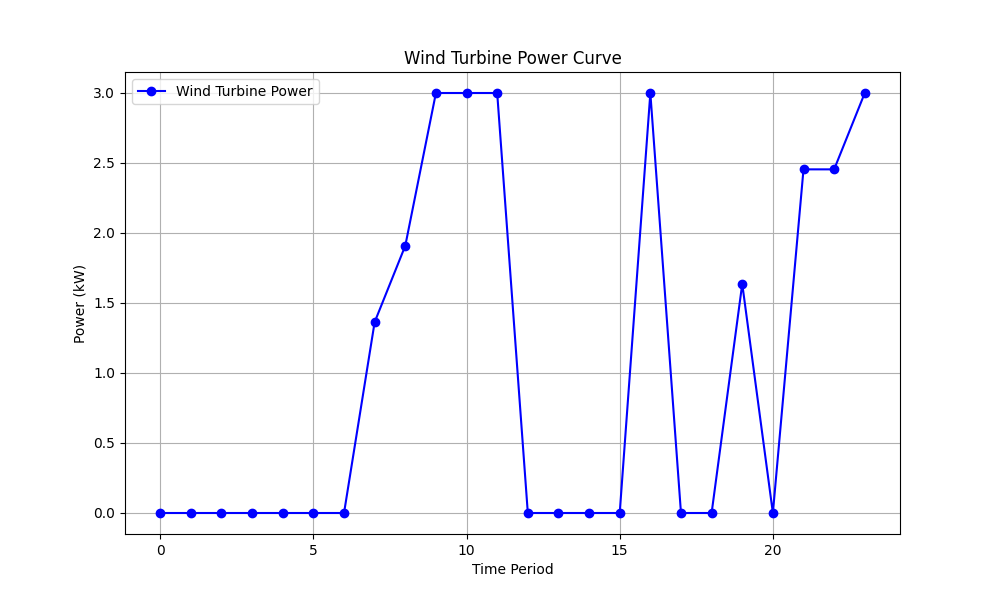
\includegraphics[width=0.8\textwidth]{figures/Figure_2.png}  % Adjust the width as needed
    \caption{Καμπύλη Ισχύος Ανεμογεννήτριας}
    \label{fig:my_label}
\end{figure}

\begin{figure}[H]  % 'H' forces the figure to stay exactly where it is placed
    \centering
    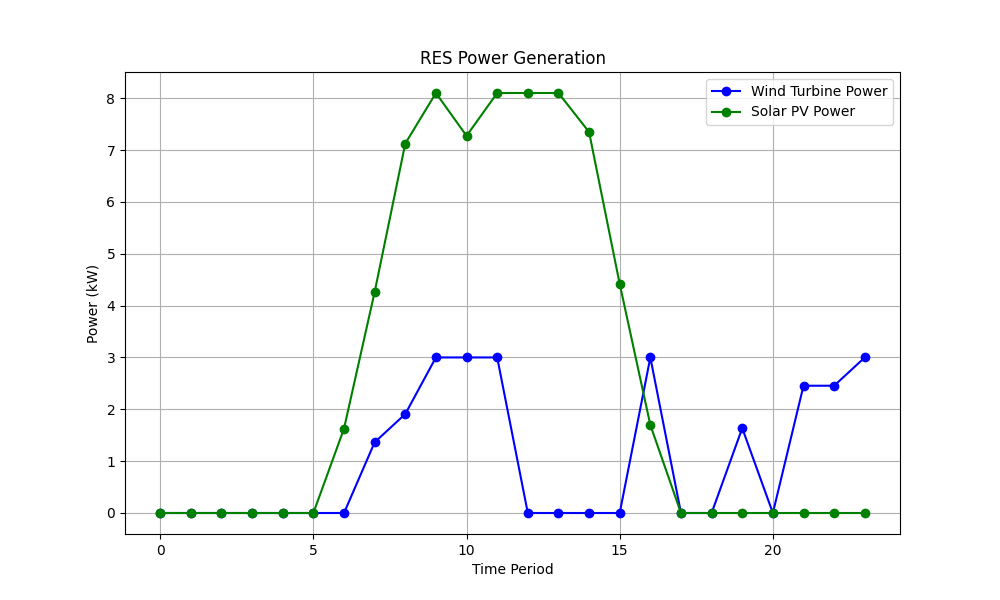
\includegraphics[width=0.8\textwidth]{figures/Figure_3.png}  % Adjust the width as needed
    \caption{Καμπύλη Ισχύος Ανανεώσιμων}
    \label{fig:my_label}
\end{figure}

Παρατηρείται ότι η παραγωγή ενέργειας κατά τη διάρκεια της ημέρας προκύπτει από τις δύο μονάδες ανανεώσιμων πηγών ενέργειας του μικροδικτύου, το σύστημα φωτοβολταϊκών πάνελ και την ανεμογεννήτρια. Η καμπύλη φορτίου ακολουθεί μία τυπική μορφή, με δύο μέγιστα. Ένα μέγιστο κατά τις πρωινές ώρες και ένα μεγαλύτερο κατά τις βραδινές ώρες. Φαίνεται πως η ισχύς που παράγεται από τα φωτοβολταϊκά πάνελ είναι σημαντικά μεγαλύτερη της ανεμογεννήτριας, γεγονός που υποδεικνύει ότι στο σύστημα θα υπάρχει περίσσεια ενέργειας, η οποία θα πρέπει να διοχετευθεί στις μονάδες αποθήκευσης. 

\begin{figure}[H]  % 'H' forces the figure to stay exactly where it is placed
    \centering
    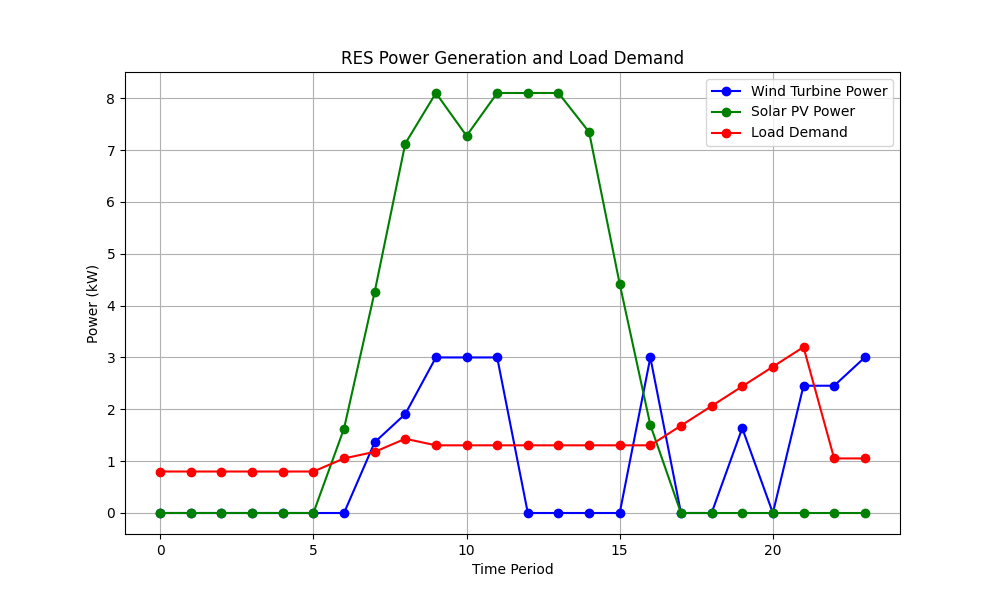
\includegraphics[width=0.8\textwidth]{figures/Figure_4.png}  % Adjust the width as needed
    \caption{Καμπύλη Παραγωγής και Καμπύλη φορτίου}
    \label{fig:my_label}
\end{figure}


\begin{figure}[H]  % 'H' forces the figure to stay exactly where it is placed
    \centering
    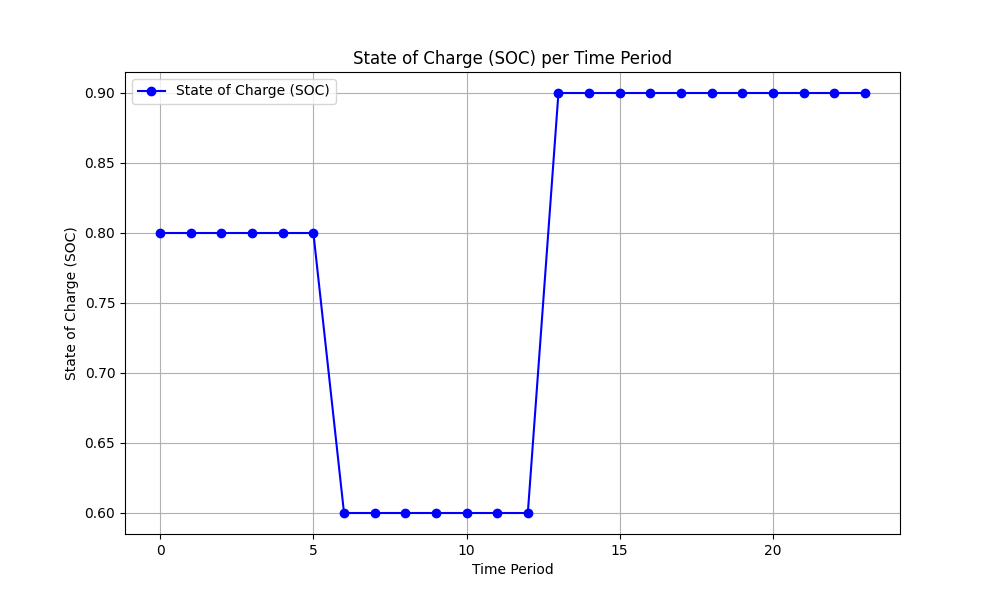
\includegraphics[width=0.8\textwidth]{figures/Figure_5.png}  % Adjust the width as needed
    \caption{Κατάσταση φόρτισης μονάδας μπαταριών}
    \label{fig:my_label}
\end{figure}

\begin{figure}[H]  % 'H' forces the figure to stay exactly where it is placed
    \centering
    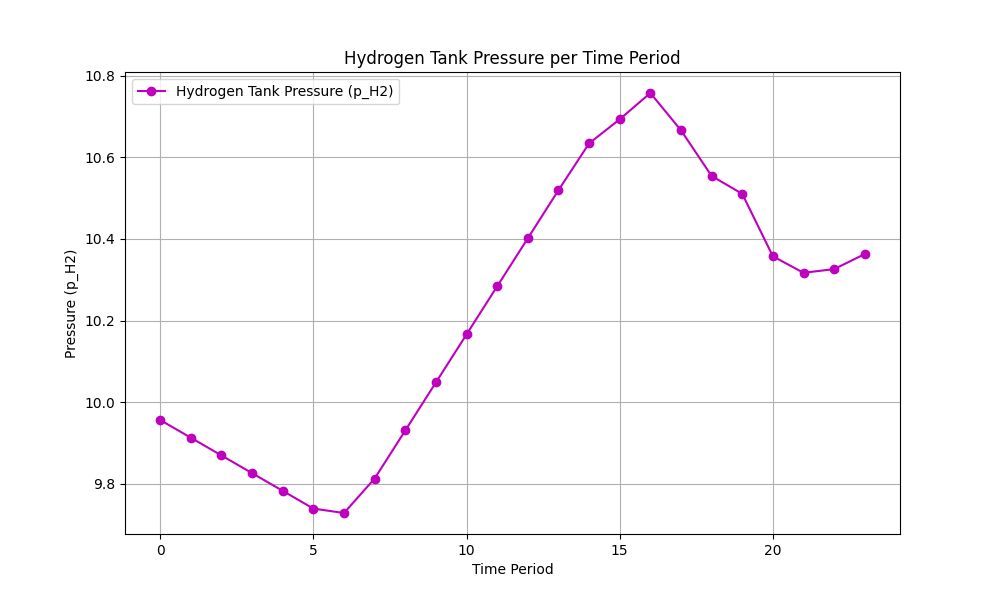
\includegraphics[width=0.8\textwidth]{figures/Figure_6.png}  % Adjust the width as needed
    \caption{Πίεση Δεξαμενής Υδρογόνου}
    \label{fig:my_label}
\end{figure}

\begin{figure}[H]  % 'H' forces the figure to stay exactly where it is placed
    \centering
    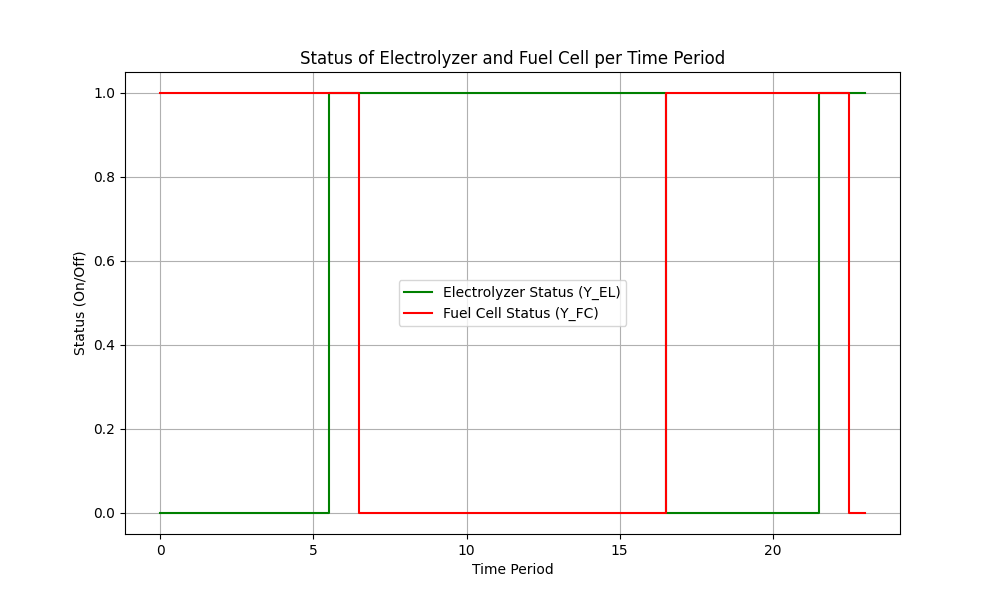
\includegraphics[width=0.8\textwidth]{figures/Figure_7.png}  % Adjust the width as needed
    \caption{Κατάσταση λειτουργίας μονάδας υδρογόνου}
    \label{fig:my_label}
\end{figure}

\subsection{Τυπική ημέρα Φθινοπώρου}
\subsection{Τυπική ημέρα Χειμώνα}
\subsection{Τυπική ημέρα Άνοιξης}

\subsection{Ειδικές περιπτώσεις}
\subsubsection{Αστοχία Μονάδων Παραγωγής}

\en
\section{Grid-connected}

\gr
\chapter*{Συμπεράσματα}
\addcontentsline{toc}{chapter}{Συμπεράσματα}  % Add List of Tables to TOC

\chapter*{Μελλοντική Έρευνα}
\addcontentsline{toc}{chapter}{Μελλοντική Έρευνα}  % Add List of Tables to TOC







\section*{ΠΑΡΑΡΤΗΜΑΤΑ}

\section{Μετεωρολογικά δεδομένα}

\begin{table}[htbp]
    \centering
    \vspace{0.5cm} % Adjust the space here as needed
    \caption{Δεδομένα θερμοκρασίας περιβάλλοντος, οριζόντιας ηλιακής ακτινοβολίας και ταχύτητας ανέμου στις 23/07/2023 στην νότια Κρήτη \cite{solcasttoolkit}}
    \label{tab:data}
    \csvautotabular{data.csv} 
\end{table}

\newpage

\section{Παράμετροι προβλήματος βελτιστοποίησης}

\begin{table}[htbp]
    \centering
    \caption{Φωτοβολταϊκό σύστημα}
    \label{tab:pv_data}
    \begin{tabular}{lcr}
    \hline
    \textbf{Φωτοβολταϊκό σύστημα} \\
    \hline
    Ονομαστική απόδοση πάνελ, $\eta_{PV,REF}$ & 18.1\% \\
    Αριθμός πάνελ, $N_{PV}$ & 36  \\
    Μέγιστη ονομαστική ισχύς πάνελ, $P_{PV,REF}$ & $0.225 kW$  \\
    Επιφάνεια πάνελ, $A_{PV}$ & $1.244 m^2$ \\
    Υλικό πάνελ & Μονοκρυσταλλικό πυρίτιο \\
    Συντελεστής θερμοκρασίας, \alpha & $-0.38\%/K$ \\
    Ονομαστική θερμοκρασία λειτουργίας μονάδας, $NOCT$ & $45^oC$ \\
    Θερμοκρασία αναφοράς πάνελ, $T_{REF}$ & $25^oC$ \\
    \hline
    \end{tabular}
\end{table} 

\begin{table}[htbp]
    \centering
    \caption{Ανεμογεννήτρια}
    \label{tab:wt_data}
    \begin{tabular}{lcr}
    \hline
    \textbf{Ανεμογεννήτρια} \\
    \hline
    Ονομαστική ταχύτητα ανεμογεννήτριας, $v_{rated}$ & $14 m/s$ \\
    Ονομαστική ισχύς ανεμογεννήτριας, $P_{rated}$ & $3 kW$ \\
    Ταχύτητα εισόδου ανεμογεννήτριας, $v_{cut-in}$ & $3 m/s$ \\
    Ταχύτητα εξόδου ανεμογεννήτριας, $v_{cut-out}$ & $18 m/s$ \\
    \hline
    \end{tabular}
\end{table} 

\begin{table}[htbp]
    \centering
    \caption{Μπαταρίες}
    \label{tab:bat_data}
    \begin{tabular}{lcr}
    \hline
    \textbf{Μπαταρίες} \\
    \hline
    Ονομαστική τάση μπαταρίας, $U_{B}$ & 12 V \\
    Ονομαστική χωρητικότητας μπαταρίας (C20), $Q_B$ & 240 Ah \\
    Αριθμός μπαταριών, $N_B$ & 32 \\
    Μπαταρίες ανά σειρά & 4 \\
    Τύπος μπαταρίας & Μολύβδου-οξέος (Lead-acid) \\
    Κόστος επένδυσης ανά μπαταρία, $C_{B,IN}$ & 400 € \\
    Μέγιστη κατάσταση φόρτισης, $SOC_{MAX}$ & 0.90 \\
    Ελάχιστη κατάσταση φόρτισης, $SOC_{MIN}$ & 0.60 \\
    Αρχική κατάσταση φόρτισης, $SOC_{IN}$ & 0.80 \\
    Μέγιστη ισχύς φόρτισης/εκφόρτισης, $P_{B,MAX}$ & 18 kW \\
    Ισοδύναμοι κύκλοι φόρτισης/εκφόρτισης, $N_{CYCLES}$ & 1300 \\
    Απόδοση συστήματος μπαταριών κατά τη φόρτιση, $\eta_{B_{CH}}$ & 0.60 \\
    Απόδοση συστήματος μπαταριών κατά την εκφόρτιση, $\eta_{B_{DIS}}$ & 0.75 \\
    Κόστος λειτουργίας \& συντήρησης, $C_{O\&M,B}}$ &  0 \\
    \hline
    \end{tabular}
\end{table}   

\begin{table}[htbp]
    \centering
    \caption{Μονάδα υδρογόνου}
    \label{tab:hyd_data}
    \begin{tabular}{lcr}
    \hline
    \textbf{Μονάδα ηλεκτρόλυσης} \\
    \hline
    Ονομαστική ισχύς μονάδας ηλεκτρόλυσης, $P_{{EL}_{REF}}$ & 6 kW \\
    Ονομαστική παραγόμενη ροή υδρογόνου ($0^oC$, $1 bar$), $V_{H_2,EL_{REF}}$ & 1.05 m^3/h \\
    Είδος ηλεκτρολύτη & πολυμερικής μεμβράνης, PEM \\
    Ελάχιστη ισχύς μονάδας ηλεκτρόλυσης, $P_{EL,MIN}$ & 1.5 kW \\
    Μέγιστη ισχύς μονάδας ηλεκτρόλυσης, $P_{EL,MAX}$ & 6.2 kW \\
    Χρόνος ζωής μονάδας ηλεκτρόλυσης, $L_{EL}$ & 30000 h \\
    Κόστος επένδυσης μονάδας ηλεκτρόλυσης, $C_{EL,IN}$ & 75000 € \\
    Κόστος λειτουργίας και συντήρησης, $C_{O\&M,EL}(t)$ & 0.2 €/h \\
    Απόδοση μονάδας ηλεκτρόλυσης, $\eta_{EL}$ & 0.7 \\
    \hline
    \textbf{Μονάδα αποθήκευσης υδρογόνου} \\
    \hline
    Μέγιστη πίεση υδρογόνου στη δεξαμενή, $p_{H_2,MAX}$ & 13.8 bar \\
    Ελάχιστη πίεση υδρογόνου στη δεξαμενή, $p_{H_2,MIN}$ & 2 bar \\
    Αρχική πίεση δεξαμενής, $p_{H_2,IN}$ & 10 bar \\
    Μέση θερμοκρασία στη δεξαμενή, $T_{H_2}$ & 313 K \\
    Συνολικό όγκος δεξαμενής υδρογόνου, $V_{H_2}$ & 4 m^3 \\
    \hline
    \textbf{Μονάδα κυψελών καυσίμου υδρογόνου} \\
    \hline
    Ονομαστική ισχύς, $P_{FC}$ & 5 kW \\
    Ονομαστική κατανάλωση υδρογόνου ($0^oC$, $1 bar$), $V_{{H_2,FC}_{REF}}$ & 3.90 m^3/h \\
    Είδος κυψέλης καυσίμου υδρογόνου & πολυμερικής μεμβράνης, PEM  \\
    Ελάχιστη ισχύς, $P_{FC,MIN}$ & 0.5 kW \\
    Μέγιστη ισχύς μονάδας, $P_{FC,MAX}$ & 6 kW \\
    Κόστος επένδυσης μονάδας, $C_{FC,IN}$ & 28000 € \\
    Χρόνος ζωής μονάδας, $L_{FC}$ & 30000 h \\
    Κόστος λειτουργίας και συντήρησης μονάδας, $C_{O\&M,FC}(t)$ & 0.2 €/h \\
    Απόδοση μονάδας κυψελών καυσίμου υδρογόνου, $\eta_{FC}$ & 0.5 \\
    \hline 
    \end{tabular}
\end{table}   

% \nocite{*} % To show all references in the bibliography

% Change bibliography language to Greek and show Greek title "Βιβλιογραφία"
\selectbiblanguage{greek}
\bibliographystyle{babplain} 
\bibliography{bibliography} 

\end{document}